\subsection{Пространства $L_p$}

\begin{note}
	В этой главе мы закрепляем за $E$ --- измеримое множество, а любая функция $f \colon E \to \sxR$ автоматически считается измеримой.
\end{note}

\begin{definition}
	Для функции $f \colon E \to \sxR$ назовём \textit{$p$-нормой} $\|f\|_p$ значение следующего выражения:
	\[
		\|f\|_p := \ps{\int_E |f(x)|^pd\mu(x)}^{1/p}
	\]
	где $p \in (0; +\infty)$. При этом мы разрешаем $p$-норме принимать бесконечное значение.
\end{definition}

\begin{reminder} (Аксиомы нормы)
	Пусть $V$ --- линейное пространство над $\R$. \textit{Нормой}\\ $\|\cdot\| \colon V \to \R_+$ на $V$ называется оператор, удовлетворяющий следующим требованиям:
	\begin{enumerate}
		\item (Невырожденность) \(\forall v \in V\ \ \|v\| = 0 \Lra v = 0\)
		
		\item (Неравенство треугольника) \(\forall v, u \in V\ \ \|v + u\| \le \|v\| + \|u\|\)
		
		\item (Линейность) \(\forall \alpha \in \R, v \in V\ \ \|\alpha v\| = |\alpha| \cdot \|v\|\)
	\end{enumerate}
	Линейное пространство с нормой называется \textit{линейно нормированным пространством}.
\end{reminder}

\begin{note}
	Наша цель --- доказать, что при $p \in \lsi{1; +\infty}$ $p$-норма действительно является нормой для пространства классов эквивалентных функций. При этом свойства 1 и 3 уже доказывались, поэтому осталось проверить неравенство треугольника.
\end{note}

\begin{note}
	Если $p \in (0; 1)$, то $\|f\|_p$ не удовлетворяет неравенству треугольника.
	
	Рассмотрим $f = \chi_{[0; 1/2]}$ и $g = \chi_{[1/2; 1]}$. Тогда $\|f\|_p = \|g\|_p = (1/2)^{1/p}$, при этом $\|f + g\|_p = 1$. Осталось посмотреть, при каких $p$ не выполнено неравенство треугольника:
	\[
		1 > \ps{\frac{1}{2}}^{1/p} \! + \ps{\frac{1}{2}}^{1/p} \Lra \ps{\frac{1}{2}}^{1/p} < \frac{1}{2} \Lra \frac{1}{p} > 1 \Lra p < 1 
	\]
\end{note}

\begin{proposition} (Неравенство Юнга)
	Пусть $p > 1$, $q > 1$ и $1 / p + 1 / q = 1$. Тогда выполнено неравенство:
	\[
		\forall a, b \ge 0\ \ a \cdot b \le \frac{a^p}{p} + \frac{b^q}{q}
	\]
\end{proposition}

\begin{proof}~
	\begin{itemize}
		\item Геометрическое доказательство. Нарисуем график $y = x^{p - 1}$, отметим на оси $x$ точку $x = a$, на оси $y$ точку $y = b$. Тогда верно неравенство \(ab \le S_1 + S_2\), где $S_1$ --- площадь под графиком до $a$, $S_2$ --- площадь над графиком до $b$.
		\begin{center}
			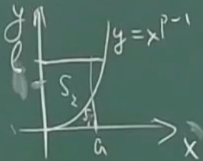
\includegraphics[width=0.4\textwidth]{images/young_inequation.png}
		\end{center}
		С одной стороны, $S_1 = \int_0^a x^{p - 1}dx = a^p / p$, а с другой стороны, $y = x^{p-1} \Lra x = y^{1 / (p - 1)} = y^{q - 1}$, то есть $S_2 = \int_0^b y^{q - 1}dy = b^q/q$, отсюда и требуемое неравенство.
		
		\item Доказательство через выпуклость $\ln x$: неравенство тривиально выполнено для $a = 0$ или $b = 0$. Иначе нам известно с первого курса, что функция натурального логарифма является выпуклой вверх. Это значит верность следующего утверждения:
		\[
			\forall a, b > 0\ \forall \alpha, \beta \ge 0, \alpha + \beta = 1\ \ \ \ln(\alpha a + \beta b) \ge \alpha\ln(a) + \beta\ln(b)
		\]
		В частности, можно рассмотреть $\alpha = 1 / p$ и $\beta = 1 / q$ и пропотенцировать это неравенство:
		\[
			\exp(\ln(a / p + b / q)) \ge \exp(\ln(a) / p + \ln(b) / q) \ \Lra \ \frac{a}{p} + \frac{b}{q} \ge a^{1/p} \cdot b^{1/q}
		\]
		Полученное неравенство эквивалентно неравенству Юнга, поскольку замены $a \mapsto a^p$ и $b \mapsto b^q$ сохраняют положительность.
	\end{itemize}
\end{proof}

\begin{theorem} (Неравенство Гёльдера)
	Для произвольных $f, g \colon E \to \sxR$ верно следующее утверждение:
	\[
		\forall p > 1, q := \frac{p}{p - 1} \quad \|f \cdot g\|_1 \le \|f\|_p \cdot \|g\|_q
	\]
\end{theorem}

\begin{proof}
	Если $\|f\|_p = 0$ или $\|g\|_q = 0$, то соответственно $f$ или $g$ равны нулю почти всюду и неравенство тривиально выполнено. Если $\|f\|_p$ или $\|g\|_q$ бесконечны, то и говорить нечего. Основной случай --- $\|f\|_p, \|g\|_q \in (0; +\infty)$. Докажем эквивалентное неравенство: $\|\tilde{f} \cdot \tilde{g}\|_1 \le 1$, где $\tilde{f} = f / \|f\|_p$, $\tilde{g} = g / \|g\|_q$. Для этого распишем эту норму по определению (и воспользуемся неравенством Юнга):
	\[
		\|\tilde{f} \cdot \tilde{g}\|_1 = \int_E |\tilde{f}| \cdot |\tilde{g}|d\mu(x) \le \int_E \ps{\frac{|\tilde{f}|^p}{p} + \frac{|\tilde{g}|^q}{q}}d\mu(x) = \frac{1}{p} \int_E |\tilde{f}|^pd\mu(x) + \frac{1}{q} \int_E |\tilde{g}|^qd\mu(x)
	\]
	Каждый из интегралов справа равен единице. Почему? Распишем один из них подробнее:
	\[
		\int_E |\tilde{f}|^pd\mu(x) = \int_E (|f| / \|f\|_p)^pd\mu(x) = \frac{\|f\|_p^p}{\|f\|_p^p} = 1
	\]
	Значит, полученная сумма равна $1/p + 1/q = 1$.  
\end{proof}

\begin{theorem} (Неравенство Минковского)
	Пусть $p \in \lsi{1; +\infty}$. Тогда $p$-норма обладает неравенством треугольника:
	\[
		\forall f, g \colon E \to \sxR\ \ \|f + g\|_p \le \|f\|_p + \|g\|_p
	\]
\end{theorem}

\begin{proof}
	Случай, когда $\|f\|_p$ или $\|g\|_p$ равны $\infty$ тривиально верен, а потому нам надо обосновать утверждение лишь при $\|f\|_p, \|g\|_p < \infty$. Проведём доказательство в 2 стадии:
	\begin{enumerate}
		\item $p = 1$. Тогда есть такая цепочка:
		\[
			\|f + g\|_1 = \int_E |f + g|d\mu(x) \le \int_E (|f| + |g|)d\mu(x) = \underbrace{\int_E |f|d\mu(x)}_{\|f\|_1} + \underbrace{\int_E |g|d\mu(x)}_{\|g\|_1}
		\]
		
		\item $p > 1$. Сначала поймём, что величина $\|f + g\|_p$ будет конечной, поскольку можно записать простую оценку:
		\[
			|f + g|^p \leq 2^p\max(|f|^p, |g|^p) \leq 2^p(|f|^p + |g|^p),
		\]
		из которой следует то же неравенство с нормами. Теперь проводить оценку нормы корректно:
		\[
			\int_E |f + g|^pd\mu(x) = \int_E |f + g| \cdot |f + g|^{p - 1}d\mu(x) \le \int_E |f| \cdot |f + g|^{p - 1}d\mu(x) + \int_E |g| \cdot |f + g|^{p - 1}d\mu(x)
		\]
		По неравенству Гёльдера каждое слагаемое можно оценить таким образом:
		\begin{multline*}
			\int_E |f| \cdot |f + g|^{p - 1}d\mu(x) \le 
			\\
			\ps{\int_E |f|^pd\mu(x)}^{1 / p} \cdot \ps{\int_E |f + g|^{q(p - 1)}d\mu(x)}^{1 / q} =
			\\
			\|f\|_p (\|f + g\|_p^p)^{1 / q} = \|f\|_p \cdot \|f + g\|_p^{p - 1}
		\end{multline*}
		Аналогично повторяем для второго и соединяем их:
		\[
			\|f + g\|_p^p \le \|f\|_p \cdot \|f + g\|_p^{p - 1} + \|g\|_p \cdot \|f + g\|_p^{p - 1}
		\]
		Если $\|f + g\|_p = 0$, то исходное неравенство тривиально верно. Иначе мы сокращаем на норму в полученном неравенстве и получаем требуемое.
	\end{enumerate}
\end{proof}

\begin{definition}
	\textit{Линейным пространством $L_p(E)$} называется пространство классов эквивалентности измеримых функций $f \colon E \to \ole{\R}$, для которых $\|f\|_p < \infty$ (эквивалентность задаётся равенством почти всюду).
\end{definition}

\begin{corollary} (из неравенства Минковского)
	$L_p(E)$ является линейным нормированным пространством, где норма есть уже определённая ранее $p$-норма.
\end{corollary}

\begin{corollary} (из неравенства Гёльдера)
	Если $E$ --- множество конечной меры, то $L_{p_2}(E) \subset L_{p_1}(E)$ при $p_1 < p_2$.
\end{corollary}

\begin{proof}
	Пусть $f \in L_{p_2}(E)$, то есть определено число $\int_E |f(x)|^{p_2} d\mu(x) \in \R$. Положим $p := \frac{p_2}{p_1} > 1$, $q := \frac{p}{p-1}$. Тогда применимо неравенство Гёльдера к функции $|f|^{p_1}$ и тождественной единице:
	\[
		\int_E |f(x)|^{p_1} d\mu(x) \leq \ps{\int_E |f(x)|^{p_2} d\mu(x)}^{\frac{1}{p}} \cdot \ps{\int_E 1^q d\mu(x)}^{\frac{1}{q}} = \ps{\int_E |f(x)|^{p_2} d\mu(x)}^{\frac{1}{p}} \cdot \mu(E)^{\frac{1}{q}}
	\]
	Раз $\mu(E) < \infty$, то и норма $f$ в $L_{p_1}(E)$ конечна.
\end{proof}

\begin{reminder}
	Последовательность точек $\{x_i\}_{i=1}^\infty$ метрического пространства $(X, \rho)$ называется \textit{фундаментальной}, если
	\[
		\forall \eps > 0 \ \exists N \in \N \such \forall m, n > N \ \rho(x_m, x_n) < \eps
	\]
\end{reminder}

\begin{reminder}
	Метрическое пространство называется \textit{полным}, если любая фундаментальная последовательность в нём является сходящейся.
\end{reminder}

\begin{reminder}
Линейное нормированное пространство $X$, обладающее полнотой по индуцированной метрике, называется \textit{банаховым}.
\end{reminder}

\begin{exercise}
Если последовательность $\{x_n\}_{n = 1}^\infty \subset (X, \rho)$ фундаментальна, то из неё можно выделить подпоследовательность $\{x_{n_k}\}_{k = 1}^\infty$ такую, что выполнено утверждение:
\[
	\forall k \in \N\ \rho(x_{n_{k + 1}} - x_{n_k}) < 2^{-k}
\]
\end{exercise}

\begin{theorem}
	При $p \ge 1$ пространство $L_p(E)$ является банаховым.
\end{theorem}

\begin{proof}
	Рассмотрим произвольную фундаментальную последовательность $\{f_n\}_{n = 1}^\infty \subseteq L_p(E)$. Тогда существует подпоследовательность $\{f_{n_k}\}_{k = 1}^\infty \subseteq L_p(E)$ такая, что
	\[
		\forall k \in \N\ \ \|f_{n_{k + 1}} - f_{n_k}\|_p < 2^{-k}
	\]
	Шаг 1: покажем, что эта подпоследовательность сходится поточечно почти всюду на $E$. Для этого положим $f_{n_0} := 0$ и запишем $f_{n_k}$ следующим образом:
	\[
		f_{n_k} = \sum_{i = 0}^{k - 1} (f_{n_{i + 1}} - f_{n_i}) \Lora \lim_{k \to \infty}f_{n_k} = \sum_{i = 0}^\infty (f_{n_{i + 1}} - f_{n_i})
	\]
	Если мы покажем, что ряд справа сходится абсолютно, то из этого будет следовать и обычная сходимость, а значит, и наличие поточечного предела $f_{n_k}$. Введём соответствующие обозначения:
	\[
		S_k := \sum_{i = 0}^{k - 1} |f_{n_{i + 1}} - f_{n_i}|; \ S := \lim_{k \to \infty} S_k
	\]
	Понятно, что $S_k$ --- неубывающая последовательность, поэтому к ней применима теорема Леви. Более того, она применима к последовательности $(S_k)^p$:
	\[
		\int_E S^p(x) d\mu(x) = \lim_{k \to \infty} \int_E S_k^p(x)d\mu(x)
	\]
	Из этого можно понять следующее: $S_k$ сходится п.в. $\Lra$ $S$ конечна п.в. $\Lra$ $S^p$ конечна п.в., а последнее будет следовать из конечности интеграла. Чтобы показать конечность интеграла, просто заметим, что справа написан предел $\|S_k\|_p^p$, который оценивается нехитрым образом:
	\[
		\|S_k\|_p \leq \sum_{i = 0}^{k - 1} \|f_{n_{i + 1}} - f_{n_i}\|_p < \|f_{n_1}\|_p + \sum_{i = 1}^{k - 1} \frac{1}{2^i} < \|f_{n_1}\|_p + 1
	\]
	Поскольку получена оценка сверху константой, предельный переход даёт требуемое, и теперь можно обозначить поточечный предел подпоследовательности $f_{n_k}$ как функцию $f$.\\
	Шаг 2: покажем, что $f$ лежит в $L_p(E)$. Для этого вспомним теорему Фату:
	\[
		\int_E |f(x)|^p d\mu(x) \leq \varliminf_{k \to \infty} \int_E |f_{n_k}(x)|^p d\mu(x)
	\]
	Любая фундаментальная последовательность в линейном нормированном пространстве ограничена, поэтому величины выше конечны, то есть $f \in L_p(E)$. \\
	Шаг 3: осталось установить, что вся последовательность сходится по норме к $f$. Снова применим теорему Фату:
	\[
		\forall m \in \N \ 
		\int_E |f_m(x) - f(x)|^p d\mu(x) \leq \varliminf_{k \to \infty} \int_E |f_m(x) - f_{n_k}(x)|^p d\mu(x)
	\]
	Если перейти к пределу по $m$, то окажется, что величина справа стремится к нулю, ведь из фундаментальности
	\[
		\forall \eps > 0 \ \exists N \such \forall m, n_k > N \ \|f_m - f_{n_k}\|_p^p < \eps
	\]
	А из этого следует, что
	\[
		\forall m > N \ \varliminf_{k \to \infty} \|f_m - f_{n_k}\|_p^p < \eps
	\]
	Что и утверждается. Значит, $0 \leq \lim_{m \to \infty} \|f_m - f\|_p^p \leq 0$ и теорема доказана.
\end{proof}